Come metodologia di sviluppo abbiamo scelto di applicare uno sviluppo agile con scrum.
Abbiamo suddiviso il lavoro in sei sprint totali, di cui: cinque, relativi all'implementazione di nuovi componenti, della durata di una settimana ciascuna. Una di circa due settimane in cui ci siamo occupati della rifattorizzazione del codice e della risoluzione di bug. Quest'ultima non è riportata all'interno dello sprint planning in quanto non aggiungeva funzionalità.

Prima di partire con l'implementazione si è tenuta una riunione preliminare in cui è stata fatta una sessione di scoping e planning in modo tale da definire i requisiti principali, redigere il product backlog e definire le stime dei tempi di sviluppo.

Inoltre, si è svolta una piccola fase di launching in cui è stata concordata da tutti i membri, l'architettura di base dell'applicazione.

\begin{figure}[H]
\centering
  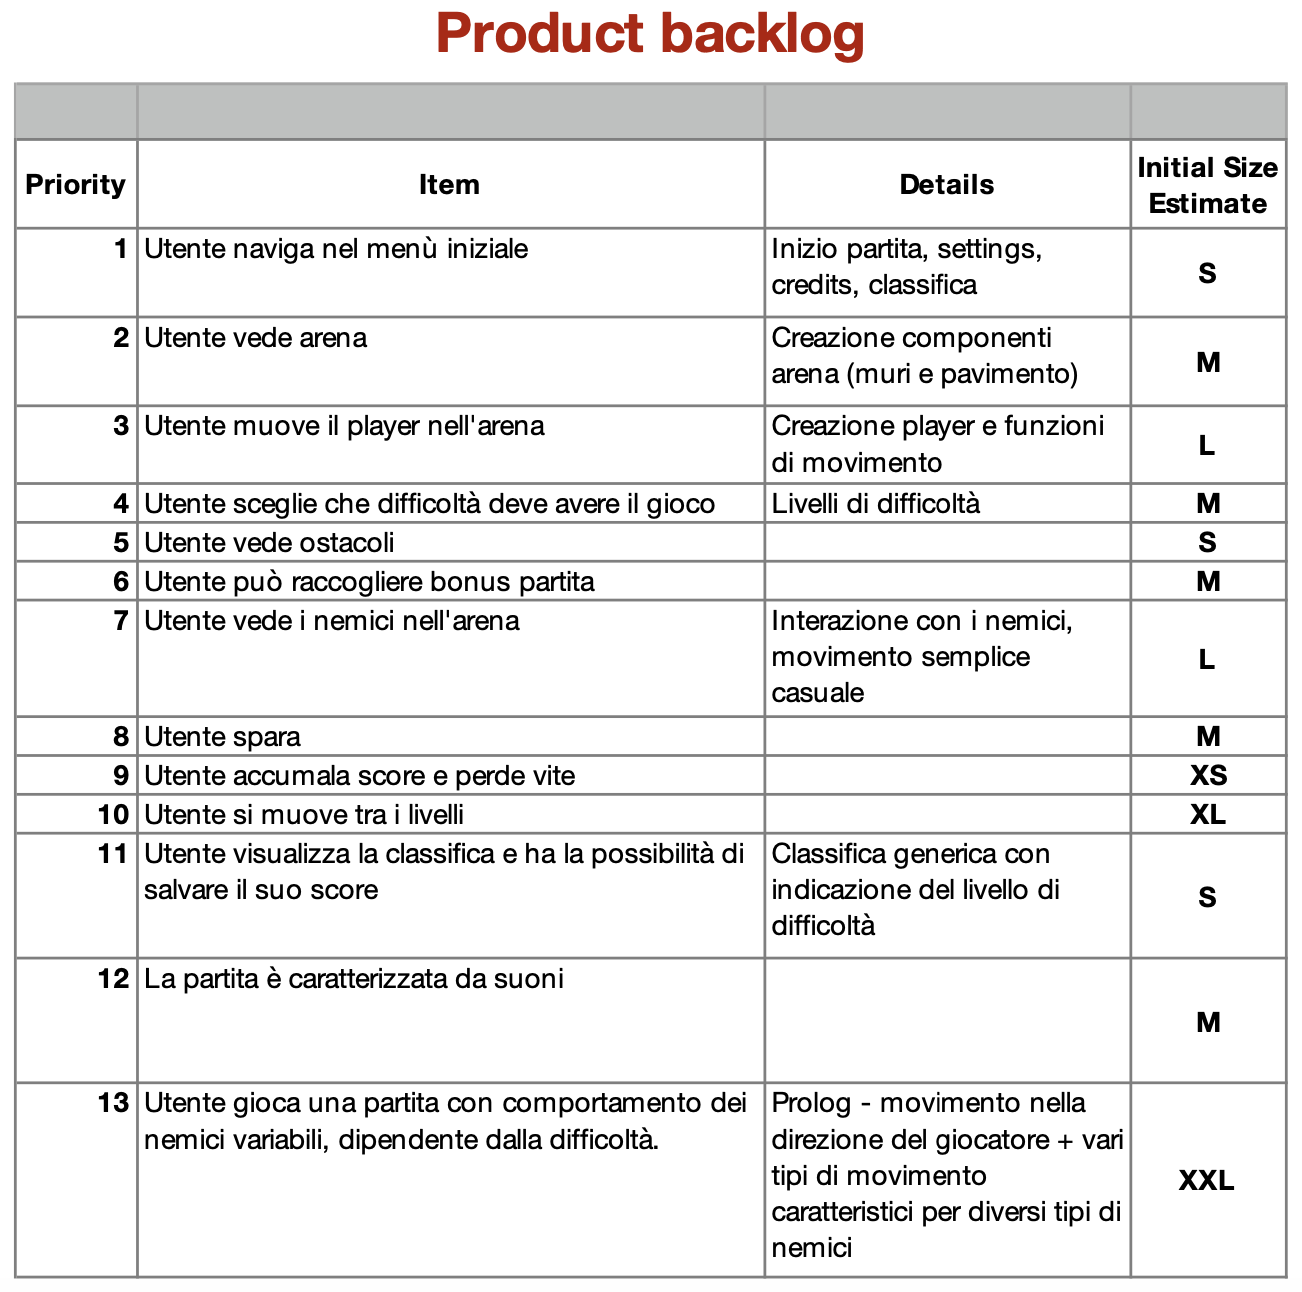
\includegraphics[width=13cm]{res/backlog.png}
  \caption{Product Backlog}
  \label{notifyAction}
\end{figure}